% For easier proof-reading, use the single-column, double-spaced layout:
\documentclass{cseminar}
% Final Paper use double-column, normal line spacing. Comment the line above and uncomment the following for the full paper
%\documentclass[cameraready]{cseminar}

\usepackage{hyperref}
\usepackage[hyphenbreaks]{breakurl}

\begin{document}

%=========================================================

\title{Something You Need To Know About Bluetooth Smart}

\author{Rui Yang\\
        Student number: 467656\\
	\texttt{rui.yang@aalto.fi}}
\maketitle

%==========================================================

\begin{abstract}
%it should include two parts:
%1. existing situation + current weakness;
%2. your contribution(a solution proposed).
Bluetooth 4.x is the latest version of Bluetooth. It embraces the feature of BLE (Bluetooth Low Energy), which is one of the reasons contributing to BLE being considered an ideal platform for Internet of Things (IoT). Compared to its previous version, BLE provides improvement of power saving, lower deployment cost and enhanced radio range, etc\cite{BLE03}. This article will focus on the evolutions of BLE from Bluetooth 4.0 to Bluetooth 4.2, the reasons behind these changes and an analysis of a special use case.

\vspace{3mm}
\noindent KEYWORDS: Bluetooth Low Energy, BLE, Bluetooth Smart

\end{abstract}

%============================================================

\section{Introduction}
Bluetooth is a wireless communication technology for short range communications especially dedicated in personal area networks (PAN). Launched to this world about 21 years ago, it has been widely implemented in our societies and provided great conveniences to our daily life. For instance, more than 2.5 billion Bluetooth products were shipped in 2013\cite{BLE04}. Benefiting from the low energy consumption of BLE, a button sized cell can provide a Bluetooth instance running with singular module for more than 3 years depending on different use cases\cite{BLE03}, which enlightens the way for a huge number of possible applications.


Since Bluetooth belongs to one kind of PANs, which means it is more connected to our body area, in addition to the significant importance and privacy of transmitted data, its protection of users' privacy and security issues naturally become the main focus of its users. Thus this article introduces the potential challenges regarding the concerns of privacy and security issues, and possible solutions.

%============================================================

\section{Background}
BLE is currently hosted by Bluetooth Special Interest Group (SIG), the design goals of which are lowest cost and easy to deploy. Since the classic Bluetooth is connection oriented, designed for data streaming in the past, it means the Bluetooth instances have to keep the connection alive even there is no data needed to be transmitted. Without the integration of sleeping mode in classic Bluetooth, this mechanism has caused it huge amount of energy consumptions. This is not good for some devices which only have  a button cell battery. In order to overcome this shortcoming of classic Bluetooth, SIG introduces Wibree of Nokia to be part of Bluetooth standard and this standard evolved to BLE later on. It mainly focuses on keeping the energy consumption as low as possible. To achieve this goal, classic Bluetooth is redesigned (not optimized from the classic Bluetooth) in BLE from radio, protocol stack, profile architecture and qualification regime\cite{BLE02}.

We may benefit a lot from the BLE. However, in some use cases, the role of classical Bluetooth cannot be replaced by BLE. For instance, as table \ref{Bluetooth_Speed} shows, being limited by the transmission speed of BLE (mainly in Basic Rate, optional in Extend Data Rate), it would no longer be suitable for some applications which require huge amount of data transmission, such as data streaming for music from a mobile phone to a headset. In order to be compatible with classical Bluetooth, BLE instance can run in either single-mode or dual-mode. The instance running in the single-mode cannot communicate with classical Bluetooth while the instance running in the dual-mode is capable of.

Moreover, the BLE has the Client/Server structure in its attribute protocol. This can allow BLE connect to the wide area network while only a gateway is needed, such as a PC or mobile devices. With the expansion of the concept of IoT, in addition to the ongoing integration of IPv6 in Bluetooth 4.2, it has been estimated that more than 2 billion units of BLE will be deployed around the globe\cite{BLE01}. The increasing popularity and huge amount of deployment\cite{BLE04} requires thorough and careful analysis of potential issues behind BLE. This is one of the reason why this article is written.

One of the major competitors of BLE is IEEE 802.15.4 known as ZigBee, which uses the same radio frequency as BLE. But the shipments of ZigBee instances are not comparable with BLE\cite{BLE05}. It mainly because ZigBee is not embedded in commonly used PCs and mobile phones whereas BLE is. With the rapid development of IoT, the shipment of BLE instances will even be bigger. From the perspective of techniques, although ZigBee is low power and its stack is quite light, BLE has even lower power and lighter stack\cite{BLE02}.

\begin{table}[t]
  \begin{center}
    \begin{tabular}{|l|lr|}
    \hline
    Bluetooth Version & Speed &\\
    \hline
    v 1.1  & 1Mbps &\\
    v 2.0  & 3Mbps &\\
    v 3.0  & 54Mbps &\\
    v 4.0  & 0.3Mbps &\\
    \hline
    \end{tabular}
    \caption{Transmission Speed Over Different Bluetooth Version}
    \label{Bluetooth_Speed}
  \end{center}
\end{table}

This article is organized as follows. Section 3 introduces the evolution of BLE essential features. Section 4 demonstrates one scenario of use cases. Section 5 presents the security features of BLE. Section 6 concludes the article.

%============================================================
\section{Evolutions of BLE Essential Features}
\subsection{Introduction to BLE}
Bluetooth Smart is described as an revolutionary technology introduced in 2010. Great conveniences have been brought to its manufacturers, developers and consumers since it emerged. According to the definition from the SIG, Bluetooth Smart is an brand name for Bluetooth version 4.0 featuring low energy consumption for the first time. So, the Bluetooth Smart is also called BLE. Compared to previous versions of Bluetooth, BLE is newly designed and has a distinct feature of low energy consumption. With the flourish of Internet of Thing (IoT) and mobile devices, it has been estimated that more 2 billion units of BLE will be deployed around the globe in 2011\cite{BLE01}. 

Normally, the design goal determines a product in respect of functionalities and performances. The goal of the classic Bluetooth is to stand by for several days or data streaming for several hours., while the BLE is designed to stand by for several years collecting or broadcasting data such as temperature and location information. In the earlier design of BLE, it is aimed to be equipped with several key features, including low cost, supporting worldwide operation, low power consumption and robustness, etc. All of these design goals determine how each sub-systems in BLE should be implemented. In order to achieve the lowest cost, the system shall be kept as small and efficient as possible and new methodologies should be adapt to boost the performance. For instance, to provide supports for new network topologies, BLE has been optimized to low the cost using research based methodology\cite{BLEDH}. In addition, BLE uses the 2.45GHz ISM band to transfer signals to support worldwide operations. However, this radio band is unlicensed and every organization can use it for commercial purpose. As a result, it is crowded with many transmission signals such as  Bluetooth and Wi-Fi. In order to co-exist in such a radio band, a mechanism called Adaptive Frequency Hopping has been introduced to help Bluetooth avoid signal conflicts. Last but not least, the low energy consumption feature has had a great impact on the design of the protocol stack of BLE. For example, the link layer has been considered as the most complicated layer in the Bluetooth protocol stacks. While in BLE, the link layer has been lightened and even provides super low energy consumption.

For a successful technology like Bluetooth, even with the revolutionary update, all the traditional features of classical Bluetooth should be included in the BLE as well. So in order to inherit all the features from previous version of Bluetooth at the same time, the BLE is designed to run in two modes: single-mode and dual-mode. In single-mode implementation, only the low energy protocol stack is implemented. In dual-mode implementation, the functionalities of BLE is integrated in classic Bluetooth controller\cite{BLEWiki}. Furthermore, one thing needed to be mentioned is its change of transmission speed. Because of the top concerns of low energy consumption, BLE commonly adopts the Basic Rate (BR) with transmission rate about 0.3 Mbps while optional with Enhanced Data Rate (EDR)(see in table \ref{Bluetooth_Speed}).

In sum, low energy, as the revolutionary feature of BLE, influenced BLE from its design to implementation. As its expanded feature, new applications shall be rising and benefits will be brought to its manufactures, developers and consumers after its ultra-high number of deployment \cite{BLE01}.

%--------------------------------------------------------------------------------------------------------
\subsection{Evolutions introduced in Bluetooth 4.1}
After the emergence of the Bluetooth Low Energy, the shipment of BLE has been on a rocket growth with 4.5 billion shipments estimated within next 5 years beginning in 2014\cite{BLE_2014}. The SIG continues to sculpt the Bluetooth 4.0 to satisfy the needs of the commercial market. So the Bluetooth 4.1, as a critical update, has been renewed its specification and assigned more flexibility for its developers to integrate more functionalities. What's more, a better co-existence with TLE radios, high transmission rate and high consistence of connections have also been included in Bluetooth 4.1. More specific details are described as follows.

As a revolutionary update to its previous version, as known as the Bluetooth 4.0, although no hardware component has been updated, Bluetooth 4.1 do provide some exciting features.
\subsubsection{Improving Usability}
To improve the consumers' usabilities which have been slightly mentioned above. The SIG defines outcomes of this specific improvements in consumer usabilities as "just work" for a simple experience. And this "just work" experience comes from the following three aspects.

First of all, Bluetooth 4.1 provides a better co-existence with TLE radios. As we all know that the LTE has been widely adopted as 4G standard for cellular networks and the global shipment of mobile phone supporting LTE also grows swiftly. In order to reduce the interference between this two promising technologies, the update in Bluetooth 4.1 allows the bluetooth device to communicate with LTE radios to minimize the interference by cooperating with each other. This is automatically done by the Bluetooth device without any operation from the user perspective.

In addition, Bluetooth 4.1 also support the seamless and silent connection between two Bluetooth devices which have been connected with each other before. This can help to improve the usability since the whole process is done automatically without any user's participation.

The third one to improve the usability is supporting bulk data transfer. The scenario is that, when large amount of data needed to be transmitted, for instance from a sensor to a roaming device, it have been implemented in Bluetooth 4.1 that techniques featuring data compression, data blocking and buffering to optimize the transfer rate. So, the transmission between two Bluetooth devices could be more efficient.

\subsubsection{Enabling Developer Innovation}
Bluetooth 4.1 enables the developer innovation in the form of allowing the developer to set the role of each Bluetooth device as a Bluetooth Smart Ready Hub and Bluetooth Smart Peripherals at the same time. As a Bluetooth Smart Ready Hub, a Bluetooth device can collect data from other Bluetooth devices. While as a Bluetooth Smart Peripheral, it can transmit the data to another Bluetooth device. By setting both roles at the same time for Bluetooth device, more use cases and applications can be built upon this innovation feature.

\subsubsection{Enabling IoT}
Bluetooth is a promising technology to provide wireless connectivity in the emerging world of IoT. With enabling IPv6 in Bluetooth 4.1, the device is considered as an IoT device after it connects to the public network using Bluetooth.
%the reason behind this update
%--------------------------------------------------------------------------------------------------------
\subsection{Evolutions introduced in Bluetooth 4.2}
Published on December 3rd in 2014, Bluetooth 4.2 continues to achieve its initial purpose which is connecting all technologies. This update is a great step forward which should be marked a milestone in the history of evolutions of Bluetooth. It is a hardware update which means to get the full functionalities of Bluetooth 4.2, one has to get a new hardware. But part of the features, including the privacy preserving, can be updated or acquired via a firmware update to the Bluetooth 4.0 and 4.1. Main updates of Bluetooth 4.2 include enhanced privacy and security, boosted transmission speed and full internet connectivity \cite{BLE_4.2}.

The goals of Bluetooth Security Manager are to provide security connections and secure the communications. As which, Bluetooth 4.2 has introduced a new security model named LE security connections \cite{BLE_SM}.  This new security model adopted an algorithm called Elliptic Curve Diffie-Man(ECDN) for public/private key generation. And a new key paring procedure has also been adopted in Bluetooth 4.1. It is claimed by the ISG that using the LE Secure Connections can protect the communication from the passive eavesdropping and Man In the Middle (MITM) attacks regardless of the paring methods \cite{BLE_SM}. More security features of Bluetooth are discussed in section 5.

Another exciting feature in Bluetooth 4.1 is its enhanced transmission rate with boosting more than 2.5 times of transmission speed and even lower transmission error \cite{BLE_4.2}. And this enhanced transmission is partially achieved by increasing the payload of transmission packet. With the increase of transmission speed, the number of packets needed to be transferred has been decreased thus less transmission errors could occur and less energy would be consumed.

In addition to the features mentioned above, from the aspect of enabling internet connectivities for IoT, if we consider Bluetooth 4.1 is a step into IoT which no longer needs an intermedia support to function as a gateway, such as a smartphone, Bluetooth 4.2 is another step forward with more new features released. Once getting the approve from the Internet Protocol Support Profile (IPSP) that Bluetooth can be allowed to directly connect to the network using IPv6/6LoWPAN, the Bluetooth can utilize the current IP structure to communicate with each other or control other devices.
%============================================================
\section{User Case Demonstration}
With the emergency of the Bluetooth, large numbers of applications based on it have been introduced to this world. This section describes one particular use case of Bluetooth in Smart Hotel. It particularly present how  the Bluetooth cooperate with other technologies and how the application is fully compatible with both the old and new version of Bluetooth.

\begin{figure}
\centering
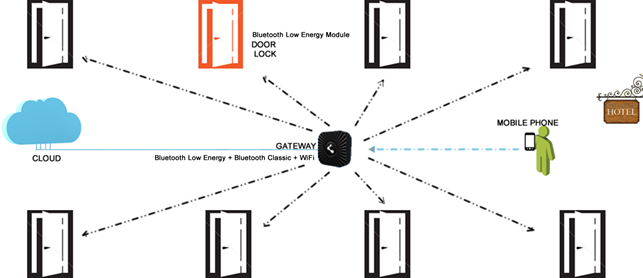
\includegraphics[width=3.5in]{figures/use_case.png}
\caption{Components in Hotel Use Cases}
\label{use case}
\end{figure}

Figure \ref{use case} shows all the components in the hotel use cases.
\\1. Mobile Devices: equipped with either classic Bluetooth or BLE;
\\2. Central Gateway Module: hardware which can connects to the Internet and communicate with classic Bluetooth or the BLE devices;
\\3. Lock modules: Physical locks embedded with BLE which control the openness of the door and communicate with the central gateway module;
\\4. Could: backend server for authentication.

The tenant holds the mobile devices and owns the credential. When they want to open their door, the mobile device connects to the central gateway module through classic Bluetooth or BLE along with user's credential. If the mobile device is using the BLE, the central gateway module then also uses the BLE to communicate with the mobile device. If the mobile device is not compatible with BLE, a classic Bluetooth connection will be created between them. Once the central gateway module received the credential from the mobile device, it forwards the credential to the backend server to verify the identity of the mobile device. Once the credential has been verified, the specific door will be opened for the tenant. So this is how the system works when tenant try to open the door. For such a system to work in the scenario of hotel, there are many technologies involved, cooperating with each other to fun as a whole. While what will be specifically focused is the role that the Bluetooth has played in this system.

In the implementation of this system, Bluetooth plays the role of providing wireless connectivity between several modules and delivering contents between them. From the beginning, the Bluetooth device in the mobile phone initializes the connection with the Bluetooth device in Central Gateway module. If the credential provided by the mobile phone has passed the verification, another Bluetooth connection will be made between the Central Gateway Module and Lock Modules of specific door. The Central Gateway Module informs the Lock Modules to open the door for the tenant. So, three Bluetooth devices have been involved in this action. The Bluetooth device acts as a Bluetooth Smart Peripheral in mobile phone within the connection with the Central Gateway Module. It transmits the data, namely the credential, and receives the response. The Bluetooth device in Lock Module acts as a Bluetooth Smart Ready Hub because it constantly listen to possible connection requests from Central Gateway Module. However, the Bluetooth device in Central Gateway module acts as both the Bluetooth Smart Ready Hub and Bluetooth Smart Peripheral. This critical feature allows it receive and send messages because the developer can define this kind of roles in the Bluetooth since BLE.

There are still numerous of applications integrated with Bluetooth device. This specific use case just simply demonstrate part of abilities that the Bluetooth is capable of. Enhanced with the newest update, Bluetooth bring great convenience to its manufactures, developers and consumers like it promised.
%============================================================
\section{Security Features}
When one Bluetooth device (Source) is communicating with another one (Target), other Bluetooth devices within their transmission range can also receive the signals transmitted between them. To create and maintain a secure Bluetooth connection is to make sure that either the message exchanged between them can not be intercepted, modified and interpreted by other anonymous devices or the message received comes from the Source that the Target trusts. With this kind of purposes, BLE has introduced several services to make it happen. For instance, Advanced Encryption Standards (AES) has been used to encrypt and decrypt the messages exchanged between BLE devices. And signature-based message signing method is used to provide and verify the identity of one message. Latter subsections describe more detailed implementation about security services in BLE.
%--------------------------------------------------------------------------------------------------------
\subsection{Encryption and Authentication services}
For two "strange" BLE devices to communicate with each other, one (Initiator) initiates a paring procedure with another device (Responder) to exchange their identity for setting up trust and getting encryption keys ready for the future data exchange \cite{BLE_SE_PAIR}. During the paring procedure, they decide which paring method should be used and what to be shared between them. After the paring procedure, all the encryption keys should have been exchanged and thus using these encryption keys to create and maintain a secure connection. The most critical step among all these three steps is what happened during paring procedure and the secure services mainly reveal in this round. The paring procedure is consists of three phases.

The first phase is two devices announcing their input and output capabilities and choosing a suitable method for phase two \cite{BLE_PAPER} (see picture \ref{Paring_method_one} and \ref{Paring_method_two}).

\begin{figure}
\centering
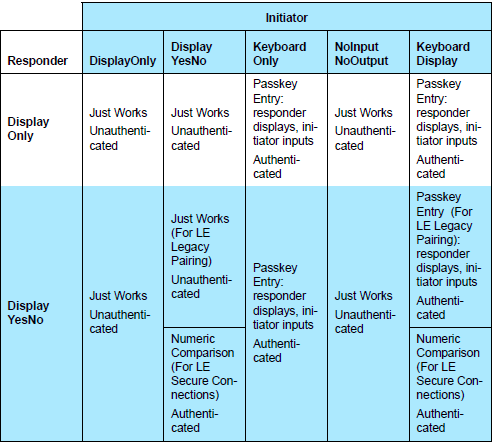
\includegraphics[width=2.5in]{figures/Paring_method_one.png}
\caption{Paring methods part one}
\label{Paring_method_one}
\end{figure}

\begin{figure}
\centering
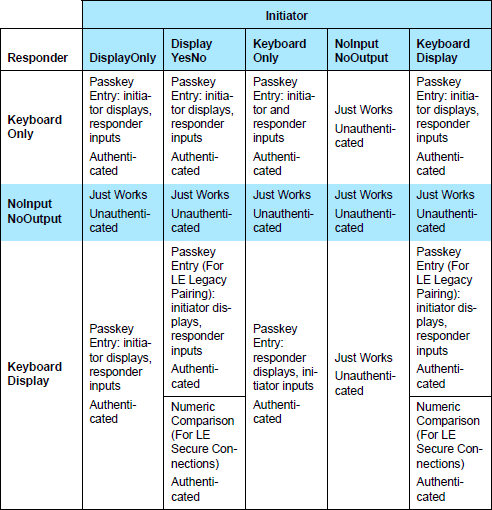
\includegraphics[width=2.5in]{figures/Paring_method_two.png}
\caption{Paring methods part two}
\label{Paring_method_two}
\end{figure}

The second phase is to make sure that the key exchange in phase three is operated in a secure way by generating a Short-Term Key (STK) to encrypt the transmission channel. The two devices agree on a Temporary Key (TK) using the method chose in the first phase. One common method that the reader might be familiar with is using the Passkey Entry method, in which the user is asked to input six random digits as the TK. Another one is assisted by other technologies (such as NFC) for the TK agreement, which is called Out of Band method. If both methods are not available, the final one called Just Works method is adopted. This method has no authentication at all and thus is lack of the ability to prevent the MITM attack. After getting the TK, the STK can be obtained for each paring devices using this algorithm: STK = AES128 (TK, Srand || Mrand).

After STK is been obtained, up to three 128-bit keys can be encrypted using STK and distributed to another device. These three keys contains  Long-Term Key (LTK), the Connection Signature Resolving Key (CSRK) and the Identity Resolving Key (IRK). LTK is used to create session key for each Link Layer connection (See BLE protocol structure in Fig. \ref{BLE_protocol_stack}). CSRK is to sign the data at the ATT Layer and IRK is to generate the private address using the known public address thus to avoid the tracking.

So, basically this is the whole three phase that the BLE 4.0 and 4.1 build trust between each other. One possible threat about this mechanism is introduced in the following section as well as the solution adopted in BLE 4.2.
\begin{figure}
\centering
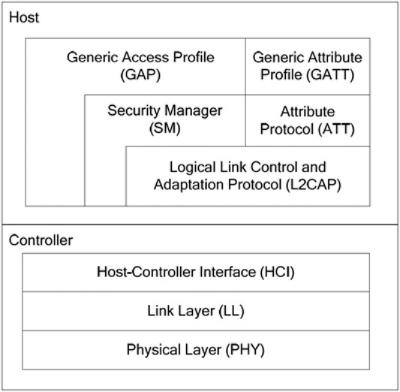
\includegraphics[width=2.5in]{figures/BLE_protocol_stack.jpg}
\caption{Bluetooth Blow Energy Protocol Stack}
\label{BLE_protocol_stack}
\end{figure}

%--------------------------------------------------------------------------------------------------------
\subsection{Possible Security Issues and Solutions}
%============================================================
\section{Conclusion}
although has been announced still need the support from OEMs to bring this benefits to the public.

%============================================================


\bibliography{seminar-paper}
\end{document}
